%-------------------------------------------------
%	Version: 0.0
%	fecha de entrega
%
%-------------------------------------------------

\documentclass[11pt]{report}

%packages
\usepackage{graphicx}
\usepackage{subcaption}

\usepackage[utf8]{inputenc}
\usepackage[spanish, es-nodecimaldot]{babel}
\usepackage{setspace}
\usepackage{ragged2e}

\usepackage{amsmath}
\usepackage{amsthm}
\usepackage{amssymb}
\usepackage{mathtools}
\usepackage{siunitx}
\usepackage[thinc]{esdiff} %derivadas faciles
\usepackage{physics} %algunos simbolos de derivadas

%path donde se encuentran las imagenes
\graphicspath{ {./figuras/} }

%---------------------------------------------------------------
%ABREVIACIONES DE COMANDOS

\theoremstyle{plain}
\newtheorem{thm}{Teorema}[chapter] % reset theorem numbering for each chapter

\theoremstyle{definition}
\newtheorem{defn}[thm]{Definición} % definition numbers are dependent on theorem numbers
\newtheorem{exmp}[thm]{Ejemplo} % same for example numbers

\newcommand{\chaptercontent}{
\section{Basics}
\begin{defn}Here is a new definition.\end{defn}
\begin{thm}Here is a new theorem.\end{thm}
\begin{thm}Here is a new theorem.\end{thm}
\begin{exmp}Here is a good example.\end{exmp}
\subsection{Some tips}
\begin{defn}Here is a new definition.\end{defn}
\section{Advanced stuff}
\begin{defn}Here is a new definition.\end{defn}
\subsection{Warnings}
\begin{defn}Here is a new definition.\end{defn}
}

\usepackage{biblatex}
%\addbibresource{Tarea1.bib}

\begin{document}

\begin{titlepage}
\title{Titulo_del_trabajo}

%-------------------------------------------------
%PORTADA
%-------------------------------------------------

	\centering
	{\scshape\LARGE Universidad Autónoma de Yucatán  \\ Facultad de ingeniería\par}
	\vspace{1cm}
	{\scshape\Large Teoría electromagnética II\par}
	\vspace{1.5cm}
	{\huge\bfseries Apuntes de clase\par}
	\vspace{0.7cm}
	{\begin{figure}[!h]
	\centering
    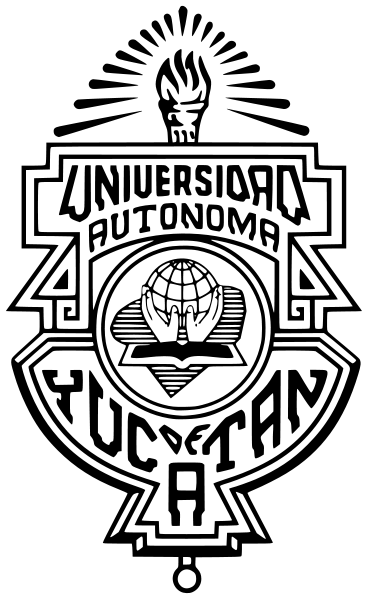
\includegraphics[scale=0.3]{UADY.png}
	\end{figure}}
	\vspace{0.7cm}
	{\Large\itshape Erick Al. Casanova Cortés\par}
	{\Large\itshape Matricula: 15014866\par}
	\vfill
	{\scshape\Large Docente\par
	Dr. O. Carvente\par}
	\vfill
	{\Large{\bfseries Fecha de modificación: \today} }

	\vfill
	
\end{titlepage}

%-------------------------------------------------
%Inicio del documento
%-------------------------------------------------

\tableofcontents

%-------------------------------------------------
%Introducción
%-------------------------------------------------

\chapter{Introducción}
\section{Formativa y sumativa}
ADAs 40 \% \\
Examenes 60 \% \\


\subsection{ADAs}
Reporte, portada, introducción, metodología, conclusiones y bibliografía, no más de una tarea por unidad, dichas tareas se recomiendan entregar en LaTex

\subsection{Exámenes}
Incluirá las tareas previas, de deberá entregar hasta una hora antes del examen.\\
Hasta dos sesiones antes del examen se llevará a cabo una sesión para resolver dudas de los problemas de la tarea.


%-------------------------------------------------
%Ley de Ampere
%-------------------------------------------------

\chapter{Ley de Ampere}

% >>>>> FIGURA

%-------------------------------------------------
%Introducción
\section{Introducción}

Hay que imaginar que dentro de un cable existe una corriente $I'$, el cual se denomina como un circuito $C'$, y en otro punto del espacio hay otra curva $C$ con una corriente $I$. ¿Cómo se mide la fuerza que $C'$ ejerce sobre $C$?\\
Se empieza definiendo un sistema de referencia, un punto del circuito donde circula $I'$ será asociado con un vector de posición $r'$ y el elemento que corre a lo largo de $C'$ se denomina como $\dd{s'}$, así a su vez para el circuito $C$ tendrán las mismas características pero no primadas. \\
Ahora lo que habrá que denominar es la fuerza a travez de la ley de Ampere. Pero ¿Como determinamos la fuerza que la corriente $I'$ que circula a lo largo del circuito definido por $C'$, ejerce sobre la corriente $I$ que circula a lo largo del circuito definido por $C$?\\


La ley de Ampere establece que:
\begin{equation}
	\vec{F}_{C' \rightarrow C} = \frac{\mu_0}{4\pi}
 \oint_C \oint_{C'} \frac{I \dd{s}\times[I' \dd{s'}\times (\vec{r}-\vec{r'})]}{|\vec{r}-\vec{r'}|^3}
 \label{eq:ley_ampere}
\end{equation}


donde $\dd{s}$ y $\dd{s'}$ son elementos diferenciales, vectoriales a lo largo de los circuitos $C$ y $C'$


¿Se cumple que $\vec{F}_{C' \rightarrow C} + \vec{F}_{C \rightarrow C'} = 0$?\\

Para eso, primero haremos una sustitución de modo que:

\begin{equation*} % 1/R
	\hat{R} = \frac{\vec{r}-\vec{r'}}{|\vec{r}-\vec{r'}|}
\end{equation*}

De modo que reescribiendo (\ref{eq:ley_ampere}) nos queda como:


\begin{equation*} %Reescribiendo
	\vec{F}_{C' \rightarrow C} = \frac{\mu_0}{4\pi}
 \oint_C \oint_{C'} \frac{I \dd{s}\times[I' \dd{s'}\times \hat{R}]}{|\vec{r}-\vec{r'}|^2}
\end{equation*}


Tomando en cuenta el triple producto vectorial, el cual nos dice que:
\begin{equation} %triple producto vectorial
	\vec{A}\times\vec{B}\times\vec{C}=\vec{B}(\vec{A}\cdot \vec{C})-\vec{C}(\vec{A}\cdot \vec{B})
	\label{eq:tiple_producto_vectorial}
\end{equation}

Otra igualdad que nos facilitaría el cálculo, podemos ver:
\begin{equation}
	\vec{\nabla}\frac{1}{r}=-\frac{\hat{r}}{r^2}
	\label{eq:gradiente_funcion_r}
\end{equation}

Entonces partiendo de \ref{eq:tiple_producto_vectorial} y \ref{eq:gradiente_funcion_r} podemos reescribir a \ref{eq:ley_ampere} como:

\begin{equation*}
	\vec{F}_{C' \rightarrow C} = \frac{\mu_0}{4\pi} \oint_{C'} \dd{s'} \oint_C \dd{\frac{1}{R}} - \frac{\mu_0}{4\pi}\oint_C \oint_{C'} \frac{\dd{s} \cdot \dd{s'}}{R^2}
\end{equation*}

Podemos ver que $\oint_C \dd{\frac{1}{R}} = 0$, por lo que otra manera de expresar a \ref{eq:ley_ampere} puede ser 


\begin{equation} %ley ampere no cruz
	\vec{F}_{C' \rightarrow C} = - \frac{\mu_0}{4\pi} \frac{\mu_0}{4\pi}\oint_C \oint_{C'} \frac{\dd{s} \cdot \dd{s'}}{R^2}
	\label{eq:ley_ampere_no_cruz}
\end{equation}


Con esto podemos ver de manera más clara que se cumple

\begin{equation*} %igualdad demostrada F + F_2 = 0
	\vec{F}_{C' \rightarrow C} = - \vec{F}_{C \rightarrow C'} 
\end{equation*}

Por lo que queda demostrada la igualdad $\vec{F}_{C' \rightarrow C} + \vec{F}_{C \rightarrow C'} = 0$\\



%-------------------------------------------------
%corriente filamental infinitamente larga
\section{Corriente filamental infinitamente larga}

%---- ejercicio ------
\section*{Ejercicio}
Determinar la fuerza que una corriente filamental infinitamente larga sobre otra corriente filamental infinitamente larga.



\textit{Respuesta}\\

Se tomará la ecuación \ref{eq:ley_ampere} para resolver el problema, en este caso analizaremos el vector de cada línea:

\begin{align*}
	\vec{r}' &= z' \hat{k}\\
	\dd{s}' &= \dd{z}'\hat{k}\\
\end{align*}

\begin{align*}
	\vec{r} &= \rho \hat{\rho} + z \hat{k}\\
	\dd{s} &= \dd{z}\hat{k}\\
\end{align*}

El triple producto nos queda como:

\begin{align*}
	II' \dd{z}\hat{k} \times [\dd{z'}\hat{k} \times [\rho \hat{\rho} + (z-z')\hat{k}]]
\end{align*}


Analizando el producto cruz de cada vector unitario

\begin{align*}
	\hat{\rho} \times \hat{\phi} &= \hat{k}\\
	\hat{k} \times \hat{\rho} &= \hat{\phi} \\
	\hat{\phi} \times \hat{k} &= \hat{\rho} 
\end{align*}


Entonces el triple producto vectorial nos queda como:

\begin{align*}
	II' \dd{z}\hat{k} \times [\dd{z'}\hat{k} \times [\rho \hat{\rho} + (z-z')\hat{k}]] = -II'\rho\dd{z}\dd{z'}\hat{\rho}
\end{align*}

y sustituyendo en la ecuación \ref{eq:ley_ampere} nos queda como:

\begin{align*}
	\vec{F}_{c'\rightarrow c} = \int_\infty^\infty \int_\infty^\infty \frac{ -II'\rho\dd{z}\dd{z'}\hat{\rho}}{(\rho^2 + (z-z')^2)^{3/2}}
\end{align*}


Podemos hacer un cambio de variable de tal modo que la ecuación nos puede quedar como:

\begin{align*}
	\begin{cases}
		z - z' &= \omega \\
		\dd{z'} &= -\dd{\omega}
	\end{cases}
\end{align*}

\begin{align*}
	\int_\infty^\infty \frac{\dd{z}}{(\rho^2 + (z-z')^2)^{3/2}} &= -\int \frac{\dd{\omega}}{(\rho^2 + (z-z')^2)^{3/2}}
\end{align*}

Haciendo un segundo cambio de variable de tal modo que:

\begin{align*}
	\begin{cases}
		\omega &= \rho \tan{\theta}\\
		\dd{\omega} &= \rho \sec^2{\theta}
	\end{cases}
\end{align*}


\begin{align*}
	-\int \frac{\rho \sec^2{\theta}\dd{\theta}}{\rho^3\sec^3{\theta}}&= -\frac{1}{\rho^2} \int \cos{\theta}\dd{\theta} \\
	&= -\frac{1}{\rho^2}\sin{\theta}
\end{align*}

Regresando a nuestra variable, vemos que $\sin{\theta} = \frac{z-z'}{\sqrt{\rho^2 + (z-z')^2}}$, entonces la integral evaluada nos queda como:

\begin{align*}
	-\frac{1}{\rho^2} \frac{z-z'}{\sqrt{\rho^2 + (z-z')^2}}|^{z' = \infty}_{z' = -\infty} &= -\frac{1}{\rho^2}[-1-1]\\
	&= \frac{2}{\rho^2}
\end{align*}

Regresando a la integral anterior tenemos

\begin{align*}
	\vec{F}_{c'\rightarrow c} &= -\frac{\mu_0II'}{4\pi}\rho\hat{\rho}\int^\infty_\infty \frac{2\dd{z}}{\rho^2}\\
	&= \frac{\mu_0II'}{2\pi\rho^2}\rho\hat{\rho}\int^\infty_\infty \dd{z}
\end{align*}


Este término es la fuerza sobre el elemento $\dd{z}$ del circuito $C$. Entonces se define la fuerza por unidad de longitud sobre el circuito $C$ como:


\begin{equation} % fuerza por unidad de longitud sobre el circuito
	f = \frac{\mu_0II'}{2\pi\rho}\hat{\rho}
	\label{eq:fuerza_por_unidad_de_longitud}
\end{equation}


%---- fin ejercicio ------

%-------------------------------------------------
% Análisis de la ecuación con el triple producto 
%vs la que solo tiene el punto
\section{Comparación de \ref{eq:ley_ampere_no_cruz} con \ref{eq:ley_ampere}}

Ahora analizaremos la fuerza entre elementos de corriente. Partiendo de:

\begin{equation}
	\vec{F}_{c'\rightarrow c} = \oint \oint \dd{\vec{F}_{c'\rightarrow c}}
\end{equation}


de tal modo que: 

\begin{align*}
	\dd{\vec{F}_{c'\rightarrow c}} = \frac{\mu_0}{4\pi} \frac{I\dd{s}\times[I'\dd{s'}\times(r-r')]}{|r-r'|^3}
\end{align*}


Si nosotros plateamos que el elemento de fuerza de tal modo que

\begin{align*}
	\dd{\vec{F}_{c\rightarrow c'}} = \frac{\mu_0}{4\pi} \frac{I'\dd{s'}\times[I\dd{s}\times(r'-r)]}{|r'-r|^3}
\end{align*}

Esto nos quiere decir que:

\begin{align*}
	\dd{\vec{F}_{c'\rightarrow c}} + \dd{\vec{F}_{c\rightarrow c'}} \neq 0
\end{align*}

Ahora si lo planteamos con \ref{eq:ley_ampere_no_cruz}

\begin{align*}
	\dd{\vec{F}_{c'\rightarrow c}} = - \frac{\mu_0}{4\pi}\frac{I\dd{s}\cdot I'\dd{s'}(r-r')}{|r-r'|^3}
\end{align*}


\begin{align*}
	\dd{\vec{F}_{c\rightarrow c'}} = - \frac{\mu_0}{4\pi}\frac{I'\dd{s'}\cdot I\dd{s}(r'-r)}{|r'-r|^3}
\end{align*}

Entonces si retomamos el análisis anterior nos queda que: 

\begin{align*}
	\dd{\vec{F}_{c'\rightarrow c}} + \dd{\vec{F}_{c\rightarrow c'}} = 0
\end{align*}

Esto es debido a que la ecuación \ref{eq:ley_ampere_no_cruz} ya toma encuenta que los circuitos están cerrados, así que en la práctica se deberá involucrar siempre \ref{eq:ley_ampere}. Por lo que nuestro estudio se centrará en el uso de dicha ecuación, ya que solo analizaremos partes del circuito.\\

% ----- ejercicio ------
\section*{Ejercicio}
Una línea y un circuito cerrado rectangular, en este caso podemos ver que la parte C y A se cancelan en el circuito, quedando solo la parte B y D, las cuales pueden ser analizadas con \ref{eq:fuerza_por_unidad_de_longitud}, entonces sustituyendo vemos que:

\begin{align*}
	f &= \frac{\mu_0II'}{2\pi\rho}\hat{\rho}\\
 &= \frac{\mu_0II'}{2\pi d}\hat{x}+ \frac{\mu_0II'}{2\pi(d+a)}\hat{x}\\
 f &= \frac{\mu_0II'}{2\pi}\frac{-a}{d(d+a)} \hat{x}
\end{align*}

Podemos ver por el signo que esta fuerza es atractiva, aunque este resiltado no está completo, ya que es una fuerza por unidad de longitud, se debe multiplicar por $B$ para tener la expresión correcta, por lo que nos queda como:

\begin{align*}
	f &= -\frac{\mu_0II'}{2\pi}\frac{ab}{d(d+a)} \hat{x}
\end{align*}


% ---- fin ejercicio ----





% ----- Tarea ------
\section{Tareas}
	\subsection{Tarea 1}
Capítulo 12: corrientes eléctricas, hacer un ensayo de las secciones 12-I, II, III

	\subsection{Tarea 2}
	
	Corrientes, encontrar la fuerza que $I'$ ejerce sobre $I$.
	
	Partiendo de (\ref{eq:ley_ampere}), tenemos que definir los vectores que vamos a utilizar, los cuales serán
	
	
	\begin{figure}[!h]
		\centering
		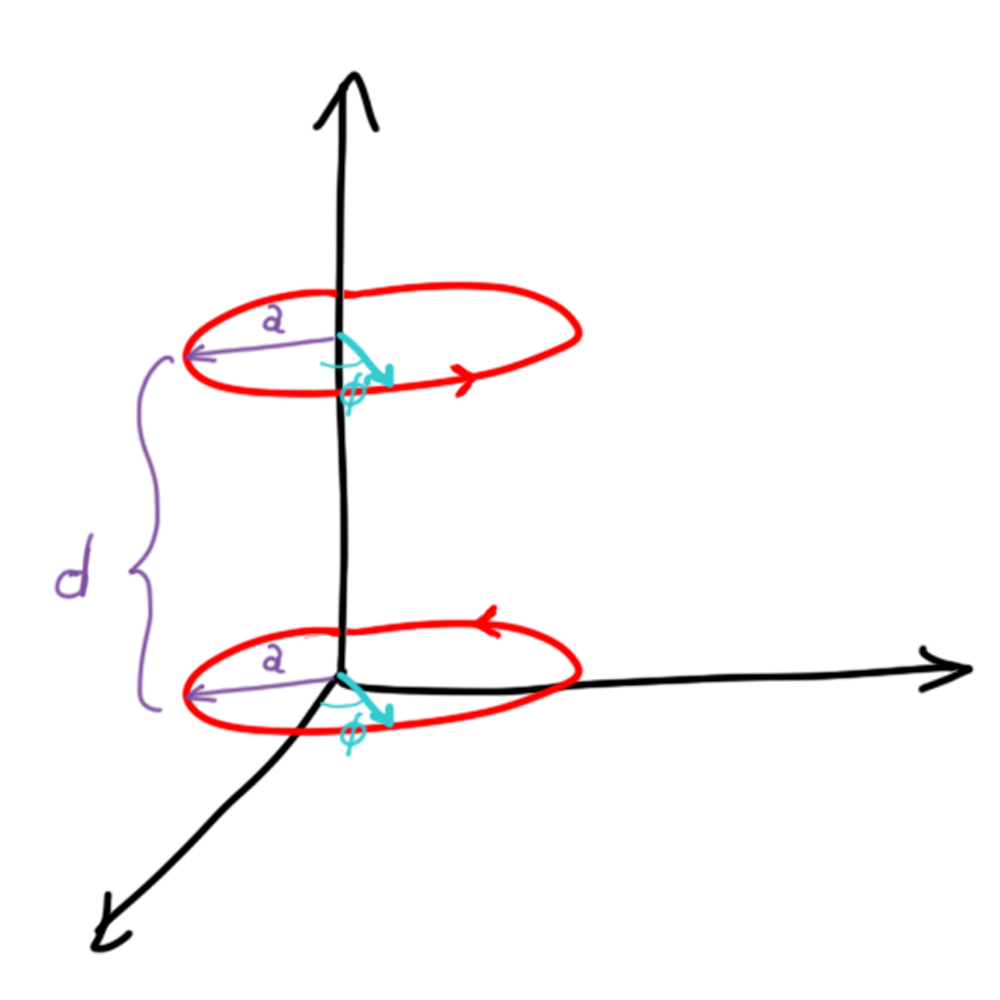
\includegraphics[scale=0.15]{Tarea2_figura.png}
		\caption{Dos circuitos}
		\label{fig:Tarea2}
	\end{figure}
	
	\begin{align*}
		\vec{r}' &= a\cos\varphi'\hat{i} + a\sin\varphi'\hat{j}\\
		\vec{r} &= a\cos\varphi\hat{i} + a\sin\varphi\hat{j}+d\hat{k}\\
	\end{align*}
	
	\begin{align*}
		\vec{r} - \vec{r}' &= a\cos\varphi\hat{i} + a\sin\varphi\hat{j}+d\hat{k} - (a\cos\varphi'\hat{i} + a\sin\varphi'\hat{j})\\
		&= a(\cos\varphi-\cos\varphi')\hat{i} + a(\sin\varphi-\sin\varphi')\hat{j} + d\hat{k}
	\end{align*}
	
	\begin{align*}
		|\vec{r} - \vec{r}'| &= \sqrt{a^2(\cos\varphi-\cos\varphi')^2 + a^2(\sin\varphi-\sin\varphi')^2 + d^2}
	\end{align*}
	
	\begin{align*}
		\dd{s'} &= a \left(-\sin\varphi'\hat{i} + a\cos\varphi'\hat{j}\right)\dd{\varphi'}\\
		\dd{s} &= a \left(-\sin\varphi\hat{i} + a\cos\varphi\hat{j}\right)\dd{\varphi'}
	\end{align*}
	
	Entonces la fuerza que ejerce $C$ sobre $C'$ es

	\begin{align*}
		\vec{F}_{C'\rightarrow C}&= \frac{\mu_0}{4\pi}\int_0^{2\pi}\int_0^{2\pi} a \left(-\sin\varphi\hat{i} + a\cos\varphi\hat{j}\right)\dd{\varphi'} \times \left[ a \left(-\sin\varphi'\hat{i} + a\cos\varphi'\hat{j}\right)\dd{\varphi'} \times \frac{(\vec{r} - \vec{r}')}{|\vec{r} - \vec{r}'|^3}\right]
	\end{align*}

La tarea es hacer la resolución de esa integral de forma numérica
%-------------------------------------------------
%Inducción magnética
%-------------------------------------------------

\chapter{Inducción magnética}

Definición de inducción magnética, partiendo de la ley de Ampere (\ref{eq:ley_ampere}) podemos agrupar los términos después del $I\dd{s}$ como $\vec{B}(r)$, de forma que:

\begin{equation}
	\vec{B}(r) = \frac{\mu_0}{4\pi}\oint_{C'} \frac{I'\dd{s'}\times\left(\vec{r}-\vec{r}'\right)}{|\vec{r}-\vec{r}'|^3}
	\label{eq:induccion_magnetica}
\end{equation}

A este término normalmente se le denomina como Ley de Biot-Savart.\\

Para el conjunto de corriente $I'_k$ circuloando a lo largo de $C_k'$, entonces \ref{eq:induccion_magnetica} se puede escribir como:

\begin{equation}
	\vec{B}_T(r) = \sum_k \frac{\mu_0}{4\pi}\oint_{C'_k} \frac{I'_k\dd{s'_k}\times\left(\vec{r}-\vec{r}'_k\right)}{|\vec{r}-\vec{r}'_k|^3}
	\label{eq:induccion_magnetica_k}
\end{equation}

Entonces la fuerza sobre un elemento de corriente $I\dd{s}$ situada en $\vec{r}$ producida por una inducción magnética:


\begin{equation*}
	\dd{F}_{C'\rightarrow I\dd{s}} = I\dd{s}\times\vec{B}(r)
\end{equation*}

Para elementos de corriente $I\dd{s}=\vec{k}\dd{a}=\vec{J}\dd{\tau}$, donde $\vec{k}$ y $\vec{J}$ son las densidades de corriente superficial y volumétrica, respectivamente:

\begin{align*}
	\vec{B}(r) &= \frac{\mu_0}{4\pi}\int_{S'} \frac{\vec{k}\times\left(\vec{r}-\vec{r}'\right)}{|\vec{r}-\vec{r}'|^3}\dd{a'}\\
	\vec{B}(r) &= \frac{\mu_0}{4\pi}\int_{V'} \frac{\vec{J}\times\left(\vec{r}-\vec{r}'\right)}{|\vec{r}-\vec{r}'|^3}\dd{\tau'}
\end{align*}

La $\vec{k}$ se toma como corriente/longitud y $\vec{J}$ tiene corriente/área


Entonces podemos ver que la fuerza se puede que ejerce 

\begin{align*}
	\vec{F}_{\vec{B}\rightarrow I } &= \oint_C I\dd{s}\times \vec{B}(r) \\
	\vec{F}_{\vec{B}\rightarrow \vec{k} } &= \oint_C \vec{k}\times \vec{B}(r) \\
	\vec{F}_{\vec{B}\rightarrow \vec{J} } &= \oint_C \vec{J}\times \vec{B}(r) \\
\end{align*}

donde

\begin{align*}%casos de B
	\vec{B} = 
	\begin{cases}
	\frac{\mu_0}{4\pi}\int_{S'} \frac{I'\dd{s'}\times\left(\vec{r}-\vec{r}'\right)}{|\vec{r}-\vec{r}'|^3}\\
	\frac{\mu_0}{4\pi}\int_{S'} \frac{\vec{k}\times\left(\vec{r}-\vec{r}'\right)}{|\vec{r}-\vec{r}'|^3}\dd{a'}\\
	\frac{\mu_0}{4\pi}\int_{V'} \frac{\vec{J}\times\left(\vec{r}-\vec{r}'\right)}{|\vec{r}-\vec{r}'|^3}\dd{\tau'}
	\end{cases}
\end{align*}


% ----- ejercicio ------

\section*{Ejercicio}

Corriente filamental de longitud finita, calcular $\vec{B}$ en un punto cualesquiera $\vec{r}$


	\begin{figure}[!h]
		\centering
		
\includegraphics[scale=0.15]{Ejercicio3.png}
		\caption{Corriente filamental}
		\label{fig:Ejercicio3}
	\end{figure}

\begin{align*} %vectores de posición
	\vec{r} &= \rho\cos{\varphi}\hat{i} + \rho\sin{\varphi}\hat{j} + z\hat{k}\\
	&= \rho\hat{\rho} + z\hat{k}\\
	\vec{r'} = z'\hat{k}
\end{align*}

\begin{align*} %diferencia de vectores de posición
	\vec{r} -\vec{r'} &= \rho\hat{\rho} + \left(z- z'\right)\hat{k}
\end{align*}

\begin{align*} %modulo de la diferencia de vectores de posición
	|\vec{r} -\vec{r'}| &= \sqrt{\rho^2 + \left(z- z'\right)^2}
\end{align*}

\begin{align*} %diferenciales
	\dd{s'} &= \dd{z}\hat{k}
\end{align*}


Partiendo de \ref{eq:induccion_magnetica}

\begin{align*} %sustitución en la ecuacion de inducción
	\vec{B} = \frac{\mu_0}{4\pi}\int_{S'} \frac{I'\dd{s'}\times\left[\rho\hat{\rho} + \left(z- z'\right)\hat{k}\right]}{|\rho^2 + \left(z- z'\right)^2|^3}
\end{align*}

Tomando el resultado de un ejercicio anterior

\begin{align*} %sol copiada xd
	\vec{B} &= \frac{\mu_0}{4\pi}\int_{S'} \frac{I'\dd{s'}\times\left[\rho\hat{\rho} + \left(z- z'\right)\hat{k}\right]}{|\rho^2 + \left(z- z'\right)^2|^3}\\
	&=  -\frac{\mu_0\rho}{4\pi}\frac{1}{\rho^2} \frac{z-z'}{\sqrt{\rho^2 + (z-z')^2}}|^{z' = L_2}_{z' = -L_1}
\end{align*}

Entonces nos queda como:

\begin{align*} %evaluando
	\vec{B} &=  -\frac{\mu_0}{4\pi\rho}\left[\frac{z+L_1}{\sqrt{\rho^2 + (z+L_1)^2}}- \frac{z-L_2}{\sqrt{\rho^2 + (z-L_2)^2}}\right]
\end{align*}


Podemos ver entonces si $L_1 \rightarrow \infty$ y $L_2 \rightarrow \infty$, entonces

\begin{align*} %viendo algo ya hecho
	\vec{B} &=  -\frac{\mu_0I'\hat{\varphi}}{4\pi\rho}
\end{align*}

% ---- fin ejercicio ----




%-------------------------------------------------
%Forma integral de la Ley de Ampere
%-------------------------------------------------

\chapter{Forma integral de la Ley de Ampere}

%-------------------------------------------------
%Potencial vectorial
%-------------------------------------------------

\chapter{Potencial vectorial}

%-------------------------------------------------
%Desarrollo multipolar del potencial vectorial
%-------------------------------------------------

\chapter{Desarrollo multipolar del potencial vectorial}

%-------------------------------------------------
%Ley de inducción de Faraday
%-------------------------------------------------

\chapter{Ley de inducción de Faraday}

%-------------------------------------------------
%Energía magnética
%-------------------------------------------------

\chapter{Energía magnética}

%-------------------------------------------------
%Magnetismo en presencia de materia y ecuaciones de Maxwell
%-------------------------------------------------

\chapter{Magnetismo en presencia de materia y ecuaciones de Maxwell}

%-------------------------------------------------
%Final del documento
%-------------------------------------------------

\end{document}
